% Created 2024-02-08 Thu 07:47
% Intended LaTeX compiler: pdflatex
\documentclass[presentation]{beamer}
\usepackage[utf8]{inputenc}
\usepackage[T1]{fontenc}
\usepackage{graphicx}
\usepackage{longtable}
\usepackage{wrapfig}
\usepackage{rotating}
\usepackage[normalem]{ulem}
\usepackage{amsmath}
\usepackage{amssymb}
\usepackage{capt-of}
\usepackage{hyperref}
\mode<beamer>{\usetheme{Madrid}}
\definecolor{SUred}{rgb}{0.59375, 0, 0.17969} % SU red (primary)
\definecolor{SUblue}{rgb}{0, 0.17578, 0.38281} % SU blue (secondary)
\setbeamercolor{palette primary}{bg=SUred,fg=white}
\setbeamercolor{palette secondary}{bg=SUblue,fg=white}
\setbeamercolor{palette tertiary}{bg=SUblue,fg=white}
\setbeamercolor{palette quaternary}{bg=SUblue,fg=white}
\setbeamercolor{structure}{fg=SUblue} % itemize, enumerate, etc
\setbeamercolor{section in toc}{fg=SUblue} % TOC sections
% Override palette coloring with secondary
\setbeamercolor{subsection in head/foot}{bg=SUblue,fg=white}
\setbeamercolor{date in head/foot}{bg=SUblue,fg=white}
\institute[SU]{Shenandoah University}
\titlegraphic{
\includegraphics[width=0.5\textwidth]{\string~/Documents/suLogo/suLogo.pdf}}
\usetheme{default}
\author{Chase Mathison\thanks{cmathiso@su.edu}}
\date{8 February 2024}
\title{The Washer Method}
\hypersetup{
 pdfauthor={Chase Mathison},
 pdftitle={The Washer Method},
 pdfkeywords={},
 pdfsubject={},
 pdfcreator={Emacs 29.1 (Org mode 9.6.7)}, 
 pdflang={English}}
\begin{document}

\maketitle

\section{Announcements}
\label{sec:org6adc040}
\begin{frame}[label={sec:org0d4f3c9}]{Announcements}
\begin{enumerate}
\item Homework in MyOpenMath
\item Make sure to come to office hours if you have questions. (Friday
via Zoom, 10 AM - 12 PM)
\item Quiz in Canvas today.
\end{enumerate}
\end{frame}

\section{The Lecture}
\label{sec:org24a316c}
\begin{frame}[label={sec:org2f91d53}]{Other solids of revolution}
Solids of revolution are a little more general than solids that always
have a circular cross section.  
For example, let's consider finding the volume of the solid generated by
rotating the region bounded by the curves
\[
y = x^2,\, y = \sqrt{x}\]
about the \(x-\)axis.
\vspace{10in}
\end{frame}

\begin{frame}[label={sec:org045b8e9}]{Other solids of revolution}
\end{frame}

\begin{frame}[label={sec:org5fa38b1}]{The washer method}
In general, the cross section of a solid of revolution will \alert{not} be
just a circle, but instead a ``washer'', or a circle with a smaller
circle cut out of the center.

Thankfully, it's still pretty easy to calculate the volume of a washer:
If the ``big'' circle has a radius of \(R\), and the ``small'' (cut out)
circle has a radius of \(r\), and the washer has a width of \(dx\),
then the volume of the washer is 
\[
 \]

From this, it's not hard to show the following.
\end{frame}

\begin{frame}[label={sec:org5395693}]{The washer method}
\begin{theorem}[The washer method]
Suppose \(f \left( x \right)\) and \(g \left( x \right)\) are
continuous, nonnegative functions with \(f \left( x \right) \ge g
\left( x \right)\) over \(\left[ a,b \right]\).  Let \(R\) denote
the region bounded above by the graph of \(f \left( x \right)\) and
below by the graph of \(g \left( x \right)\), and by the lines \(x=a\) and \(x=b\).  Then, the volume of the solid generated by rotating
\(R\) about the \(x-\)axis is given by
\[
 \]
 \phantom{butts}

\phantom{butts}
\end{theorem}
\end{frame}

\begin{frame}[label={sec:orga882c07}]{Example}
Find the volume of the ``napkin ring'' generated by rotating the region
bounded above by \(y = \sqrt{4-x^2}\), and below by \(y = 1\) about
the \(x-\)axis.

\begin{center}
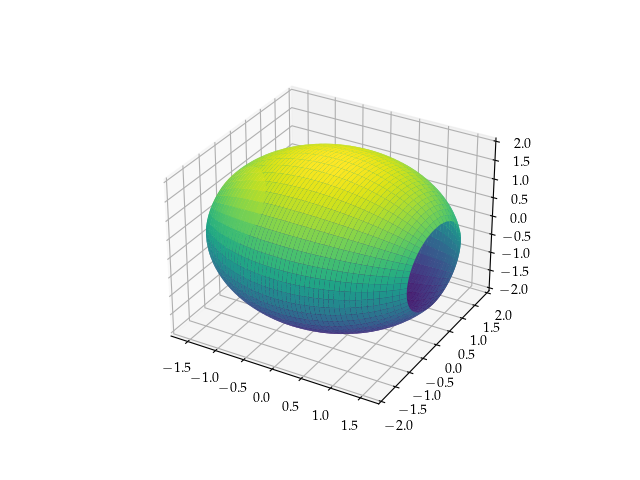
\includegraphics[width=0.5\textwidth]{../img/day007-ex02.png}
\end{center}
\vspace{10in}
\end{frame}

\begin{frame}[label={sec:org3c557a7}]{Example}
\end{frame}

\begin{frame}[label={sec:org9885078}]{Example}
Find the volume of the solid generated by rotating the region bounded
above by the graph of \(y = x\), below by the graph of \(y = 1/x\)
and on the right by \(x = 4\) about the \(x-\)axis.

\begin{center}
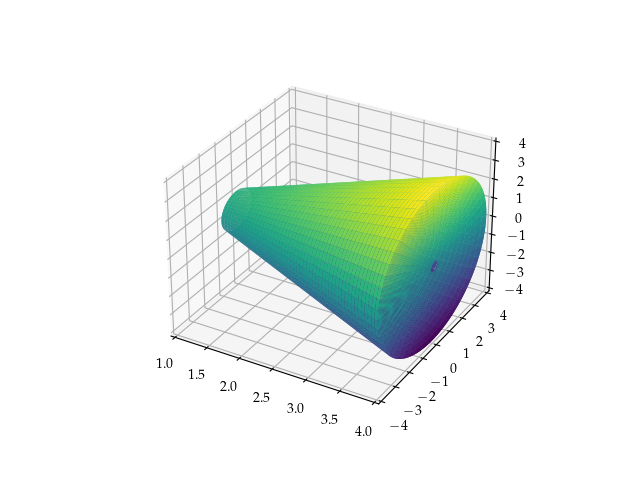
\includegraphics[width=0.5\textwidth]{../img/day007-ex03.png}
\end{center}
\vspace{10in}
\end{frame}

\begin{frame}[label={sec:org8850210}]{Example}
\end{frame}

\begin{frame}[label={sec:org969c024}]{The washer method, again}
Just like when we learned the disk method, we were also able to apply
it to volumes of revolution rotated about the \(y-\)axis, we can also
apply the washer method to volumes generated by rotating regions about
the \(y-\)axis with very little change.
\begin{theorem}[The washer method (for functions of \(y\))]
Suppose \(f \left( y \right)\) and \(g \left( y \right)\) are
continuous, nonnegative functions with \(f \left( y \right) \ge g
\left( y \right)\) over \(\left[ c,d \right]\).  Let \(Q\) denote
the region bounded on the right by the graph of \(f \left( y \right)\) and
on the left by the graph of \(g \left( y \right)\), and by the lines \(y=c\) and \(y=d\).  Then, the volume of the solid generated by rotating
\(Q\) about the \(y-\)axis is given by
\[
 \]
 \phantom{butts}

\phantom{butts}
\end{theorem}
\end{frame}

\begin{frame}[label={sec:org3d1510c}]{Example}
Find the volume of the solid generated by rotating the region bounded
on the right by the graph of \(x = \cos y\), on the left by \(x =
\sin y\) and below by \(y = 0\) about the \(y-\)axis.

\begin{center}
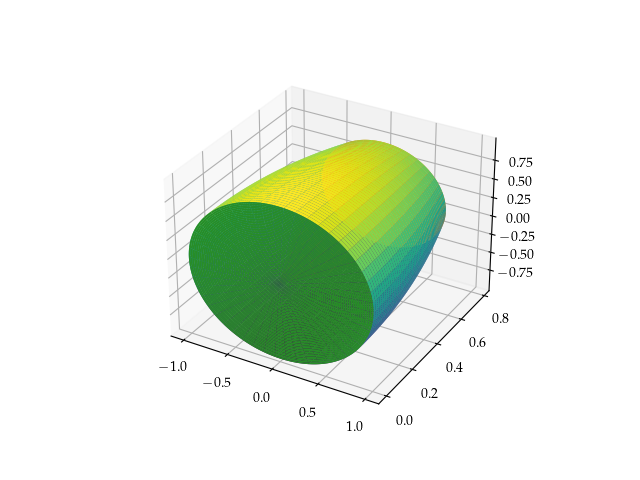
\includegraphics[width=0.5\textwidth]{../img/day007-ex04.png}
\end{center}
\vspace{10in}
\end{frame}

\begin{frame}[label={sec:org3c0e00e}]{Example}
\end{frame}

\begin{frame}[label={sec:org2071299}]{Example}
BUT WHY JUST THE \(x-\) AND \(y-\) AXES?????

We can even find the volume of a solid that is generated by rotating a
region about any vertical or horizontal line.

Let's try to find the volume of the solid generated by rotating the
region bounded by the graphs of \(y = x\) and \(y = x^2\) about the
line \(x = 2\).

\vspace{10in}
\end{frame}

\begin{frame}[label={sec:org86a62b9}]{Example}
\end{frame}

\begin{frame}[label={sec:org75a366e}]{Next time}
There's one final method that we can use to find these volumes of
revolution: cylindrical shells.  We'll learn how to use this method
next time.
\end{frame}
\end{document}